
\chapter{Experiment Results and Discussions}
%\chaptermark{EM algorithm}
\HRule \\[-0.5cm] % Horizontal line
\lhead{\emph{\textbf{Chapter3:} Experiment Results and Discussions}}

%----------------------------------------------------------------------------------------
%	SECTIONS
%---------------------------------------------------------------------------------------
\begin{spacing}{0.5}
%\begin{document}
% \vspace{-5mm}
\section{Experimental Setup}
The system was built with tunable hidden layers and number of Gibbs sampling iterations (k). It has been observed that keeping $k=1$ is sufficient to gain good performance and that varying it showed no visible improvement in the plots. A binary-binary RBM has been (BB-RBM) used, to perform a pattern storage task.
% \vspace{-5mm}
\section{Database Description}
The standard MNIST handwriting dataset was used, quantised to a binary level to emulate a binary random data set of 784 dimensions.
\begin{figure}[h]
    \centering
    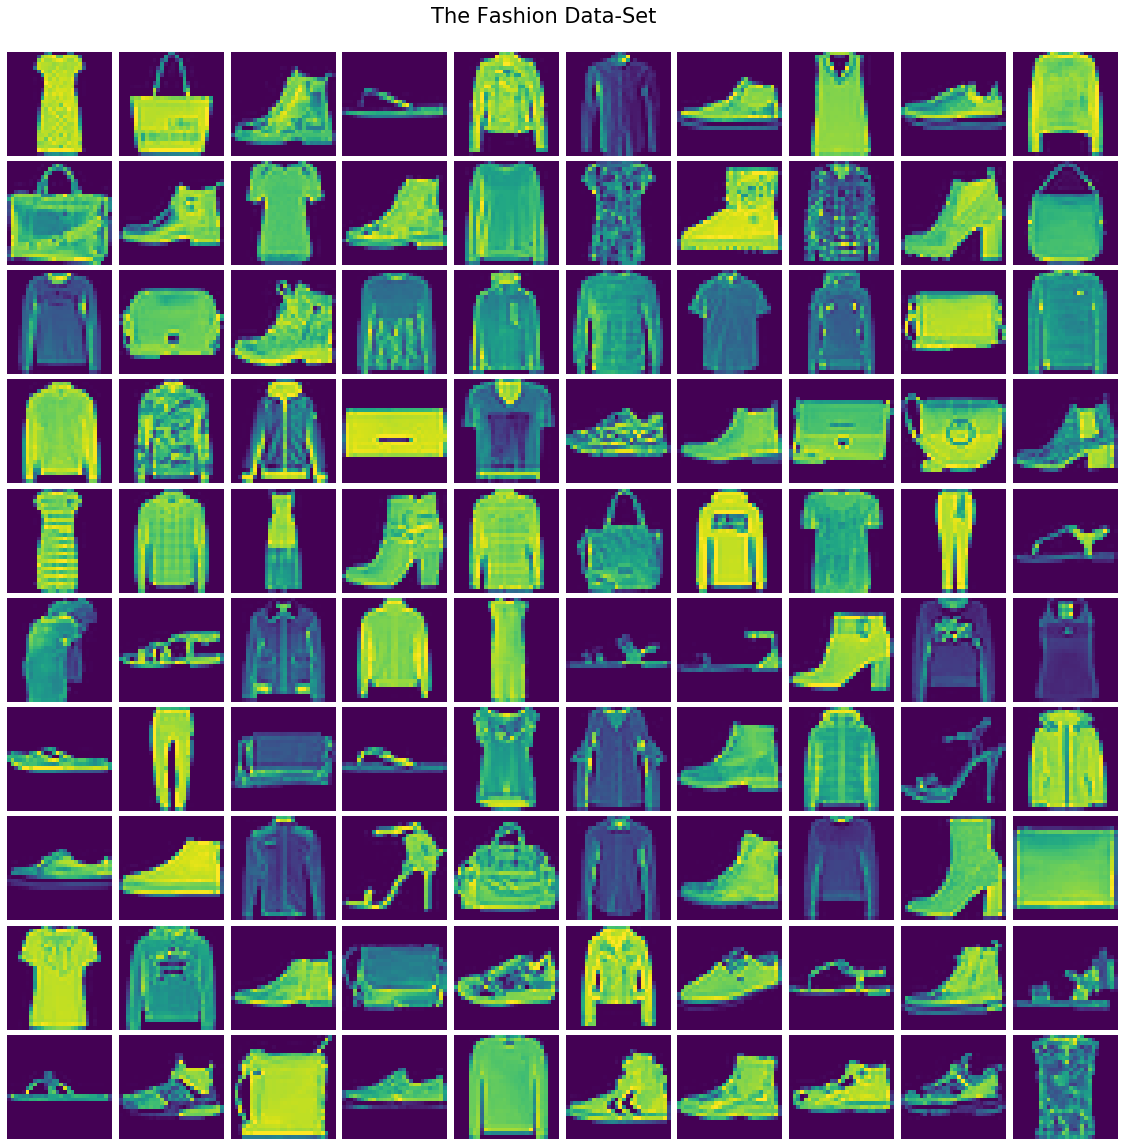
\includegraphics[scale=0.20]{Results/MNIST_DATASET.png}
    \caption{The Quantized MNIST dataset}
    \label{fig:my_label}
\end{figure}\\
\newpage
\vspace{-10mm}
\section{Results and Discussions}

\subsection{Using a 100 Hidden Layer Neurons}

\begin{figure*}[htp]
  \hspace*{-15mm}
  \subfigure[ ]{\includegraphics[scale=0.21]{Results/H_100/MNIST_348.png}}\quad
  \hspace*{+10mm}
  \subfigure[ ]{\includegraphics[scale=0.21]{Results/H_100/WEIGHTS_348.png}}

  \hspace*{-15mm}
  \subfigure[ ]{\includegraphics[scale=0.21]{Results/H_100/MNIST_FULL.png}}\quad
  \hspace*{+10mm}
  \subfigure[ ]{\includegraphics[scale=0.21]{Results/H_100/WEIGHTS_FULL.png}}
  \caption{ Figures (a) and (c) show the outputs of an RBM trained on the digits [3,4,8] and [0-9], respectively. Figures (b) and (d) show the weights between inputs and hidden layers, as an image, for these two cases.  }
\end{figure*}

\newpage

\subsection{Using 49 Hidden Layer Neurons}

\begin{figure*}[htp]
  \hspace*{-15mm}
  \subfigure[ ]{\includegraphics[scale=0.21]{Results/H_49/MNIST_348.png}}\quad
  \hspace*{+10mm}
  \subfigure[ ]{\includegraphics[scale=0.21]{Results/H_49/WEIGHTS_348.png}}

  \hspace*{-15mm}
  \subfigure[ ]{\includegraphics[scale=0.21]{Results/H_49/MNIST_FULL.png}}\quad
  \hspace*{+10mm}
  \subfigure[ ]{\includegraphics[scale=0.21]{Results/H_49/WEIGHTS_FULL.png}}
  \caption{ Figures (a) and (c) show the outputs of an RBM trained on the digits [3,4,8] and [0-9], respectively. Figures (b) and (d) show the weights between inputs and hidden layers, as an image, for these two cases.  }
\end{figure*}

\newpage

\subsection{Using 9 Hidden Layer Neurons}

\begin{figure*}[htp]
  \hspace*{-15mm}
  \subfigure[ ]{\includegraphics[scale=0.21]{Results/H_9/MNIST_348.png}}\quad
  \hspace*{+10mm}
  \subfigure[ ]{\includegraphics[scale=0.21]{Results/H_9/WEIGHTS_348.png}}

  \hspace*{-15mm}
  \subfigure[ ]{\includegraphics[scale=0.21]{Results/H_9/MNIST_FULL.png}}\quad
  \hspace*{+10mm}
  \subfigure[ ]{\includegraphics[scale=0.21]{Results/H_9/WEIGHTS_FULL.png}}
  \caption{ Figures (a) and (c) show the outputs of an RBM trained on the digits [3,4,8] and [0-9], respectively. Figures (b) and (d) show the weights between inputs and hidden layers, as an image, for these two cases.  }
\end{figure*}

% \begin{figure}[h]
%     \centering
%     \includegraphics[scale=0.20]{Results/H_100/MNIST_348.png}
%     \caption{The quantized MNIST dataset}
%     \label{fig:my_label}
% \end{figure}

% \begin{figure}[h]
%     \centering
%     \includegraphics[scale=0.20]{Results/H_100/MNIST_FULL.png}
%     \caption{The quantized MNIST dataset}
%     \label{fig:my_label}
% \end{figure}
% \section{Summary}


\end{spacing} 